
\chapter{Deep Learning Approach}

\label{Chapter4}

%----------------------------------------------------------------------------------------

In the previous chapters we have introduced the key components of the approach we followed in our study: on the one hand, we have discussed Deep Learning and how it works, and on the other, we have described existing datasets and introduced the actual data we will consider. Now, we are ready to describe our approach, the image feature extraction, the model architecture and the training scenario.

\section{Image features}

In order to train a model based on images, features need to be extracted.

\subsection{Traditional image features}

Traditionally, image feature extraction was based on a set of hand-crafted detectors for edges (Sobel), corners, blobs (LoG, DoH) and other feature descriptors (SIFT, SURF, HOG)

\begin{itemize}
	\item \url{https://en.wikipedia.org/wiki/Feature_detection_(computer_vision)}
	\item \url{https://en.wikipedia.org/wiki/Scale-invariant_feature_transf1orm}
	\item \url{https://en.wikipedia.org/wiki/Speeded_up_robust_features}
	\item \url{https://en.wikipedia.org/wiki/Histogram_of_oriented_gradients}
\end{itemize}

\textcolor{red}{(briefly describe, add proper references)}

\subsection{NN features and transfer learning}

Recent approaches to image classification using Neural Networks have benefited from increasing computational power, and deep Convolutional Neural Networks have been able to achieve high performance. 

Training a deep CNN from scratch requires a big and exhaustive dataset along with a huge amount of computational power, but it has been shown that the architectures of pre-trained NN can be reused for other purposes and achieve an equally great performance. Consequently, there is an increasing library of available pre-trained models and weights: Xception, VGG, InceptionV3, ResNet.

Most of these models have weights pre-trained on ImageNet, a large dataset containing more than 14 million hand-annotated images and over 20.000 categories.

These pre-trained architectures can be re-purposed by reusing the learned weights and either replacing the final layers of the net by some other classifier, or even fine-tuning all the layers for the given problem. In any case, the initial layers of the Neural Network provide a great image feature extractor.

\begin{figure}[h!]
	\centering
	\captionsetup{width=1\linewidth}
	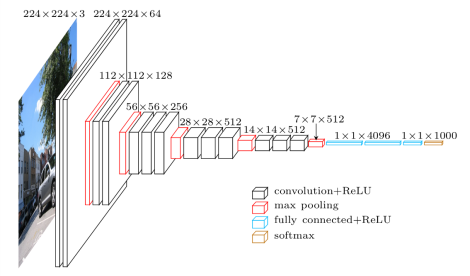
\includegraphics[width=1\textwidth]{Figures/imagenet_vgg16.png}
	\caption{\textbf{VGG16 architecture}. Stack of $3\times 3$ convolutional and max pooling layers.}
	\label{fig:degrade}
\end{figure}

\begin{itemize}
	\item VGG: \url{https://arxiv.org/abs/1409.1556}
	\item \url{https://iopscience.iop.org/article/10.1088/1742-6596/1087/6/062032/pdf}
	\item \url{https://arxiv.org/abs/1805.02294}
	\item \url{https://cs.nyu.edu/~fergus/papers/zeilerECCV2014.pdf}
	\item \url{https://towardsdatascience.com/transfer-learning-from-pre-trained-models-f2393f124751}
	\item \url{https://www.mitpressjournals.org/doi/pdf/10.1162/neco_a_00990}
	\item \url{http://www.image-net.org/}
	\item \url{https://en.wikipedia.org/wiki/ImageNet}
	\item \url{https://keras.io/applications/}
\end{itemize}

\subsection{ResNets}

Experience with Neural Networks, and CNN in particular, show that deeper nets tend to perform better, as these are more capable to model higher complexity. Yet, at some depth point, training becomes too difficult, because the gradient values obtained from the loss function are lost after several layers. This is known as \textbf{vanishing gradient}. Res

\textcolor{red}{architecture (image), training set, etc}

\begin{itemize}
	\item \url{https://towardsdatascience.com/review-resnet-winner-of-ilsvrc-2015-image-classification-localization-detection-e39402bfa5d8}
	\item \url{https://towardsdatascience.com/deep-convolutional-neural-networks-ccf96f830178}
	\item \url{https://towardsdatascience.com/understanding-and-visualizing-resnets-442284831be8}
	\item \url{https://en.wikipedia.org/wiki/Residual_neural_network}
	\item \url{https://arxiv.org/abs/1512.03385}
\end{itemize}

\section{Proposed architecture}

\subsection{resnet activations}

\textcolor{red}{images of activations (at several layers?)}

\begin{itemize}
	\item \url{}
\end{itemize}

\subsection{complete architecture}

architecture

\subsection{training}

cross validation
